\chapter{特徵參數擷取}
\label{ch:feature-extraction}
本章節將對實驗中所使用之特徵擷取方法做詳細說明。
第~\ref{sec:mfccfe}~小節將說明梅爾倒頻譜參數的特徵擷取流程。
第~\ref{sec:teccfe}~小節則說明~Teager~能量倒頻譜參數的實作方法。 

\section {梅爾倒頻譜參數}
\label{sec:mfccfe}
由於梅爾倒頻譜參數充分的考慮人耳在不同頻率的聽覺特性,
成為自動語音辨識中最常使用的特徵參數。
而梅爾倒頻譜參數的流程如圖~\ref{fig:flow_tecc_mfcc},其說明如下:    
\begin{enumerate}
\item 音框化~(framing)~:
由於語音訊號是時變的訊號,我們很難以線性非時變的方法分析長時間~(long-term)~的語音訊號特徵。
因此我們藉由音框化將其分割為短時間~(short-term)~的訊號,使得語音訊號具備暫時穩定的特性。
然而為了避免相鄰兩音框的變化過大,我們會讓相鄰音框之間有重疊的區域。
\item 預強調~(pre-emphasis)~:
為一高通濾波器~(High-pass filter),主要功用是加強聲波高頻的能量。
人類說話的聲音受到聲帶及嘴唇的效應,產生的語音在高頻部分會有衰減的特性,
透過預強調可以補償語音信號受到發音系統所壓抑的高頻部分,其如方程式(\ref{eq:pe})
\begin{equation}
\label{eq:pe}
    s_{pe}[n] = s[n] - \alpha ~ s[n-1],
\end{equation}
其中~$s_{pe}[n]$~為預強調處理過的輸出訊號,$s[n]$~為原始輸入訊號,$\alpha$~為預強調的參數~(本論文中設定為~$0.97$~)。

\item 漢明窗~(Hamming window)~:	
每個音框根據固定時間點切割會造成音框邊緣出現訊號不連續的現象,
而這種現象會造成音框經由快速傅立葉轉換後產生高頻雜訊。
為了降低雜訊的產生,我們將預強調後的音框做快速傅立葉轉換前會先乘上一個漢明窗,
以增加音框左右兩端的連續性,如方程式(\ref{eq:hammwin})。
\begin{equation}
\label{eq:hammwin}
    s_{hw}[n] = w[n] s_{pe}[n],
\end{equation}
  其中~$w[n]$~為漢明窗,式子如下
  \[
	w[n] \triangleq 0.54-0.46 \cos \left( 2\pi \left(\frac{n+0.5}{N} \right) \right),
  \]  
  其中~$N$~音框取樣數。
\item 快速傅立葉轉換~(fast Fourier transform, FFT)~:
語音訊號在時域上的變化十分快速且隨著時間不斷的改變,因此從時域上是很難觀察出它的特性。
但是在頻域上短時間內的語音訊號是呈現週期性的,
所以通常會經由快速傅立葉轉換將語音訊號轉換至頻域,觀察各個頻帶間能量的分佈,
並藉由能量的分佈找出代表不同語音的特性。
而快速傅立葉轉換方程式為
\begin{equation}
\label{eq:fft}
   X(k) = \sum_{n = 0}^{N-1}  s_{hw}[n] \exp \left( -j \frac{2 \pi kn}{N} \right) ,~0 \leq k < N. 
\end{equation}

\item 梅爾頻譜濾波器~(Mel-frequency filter bank)~:
人耳對於頻率的變化在高頻與低頻時的敏感度不同,在低頻時人耳的感受會比較敏銳,此時對頻率變化的感受就會呈線性的。
而當頻率變化位於高頻部分,人耳的感受就會越來越粗糙,當頻率大於~$1$~KHz時,人耳對於頻率的感受就會呈現對數變化。
梅爾頻率的目的即是模擬此種現象,梅爾頻率和一般頻率~$f$~的關係式為
\begin{equation}
\label{eq:mel}
	Mel(f) = 2595 \log _{10} \left( 1 + \frac{f}{{700}} \right).
\end{equation}

\item 對數壓縮~(Logarithm)~:
音波振動透過空氣經由外耳與中耳藉由三小聽骨傳遞到後方的內耳。
在傳遞的過程中,造成能量的損失,而能量最主要影響的將是人耳對於音量大小的解析度。
因此我們透過對數運算對音量壓縮,除去語音訊號在相位~(phase)~上的變化。
在此我們將梅爾頻率濾波器組中的能量取對數壓縮表示為~$s_{\log}[m]$。

\item 離散餘弦轉換~(discrete cosine transform, DCT)~:
在對數壓縮後經由離散餘弦轉換的目的是希望將訊號轉換為倒頻譜係數。
其主要用意在於減少維度間的關係,有助於隱藏式馬可夫模型在儲存共變異矩陣時資料的縮減,增加辨識效率。
方程式如下
\begin{equation}
\label{eq:dct}
  c_i = \sum_{m=1}^{M} s_{\log}[m] \cos \left[ \frac{ \pi i \left( m-0.5 \right) }{M} \right],
\end{equation}
其中~$c_i$~為~MFCC~特徵向量,$M$~為濾波器的個數。
\end{enumerate}

\begin{figure}[!htb]
\centering
\includegraphics[width=1.0\textwidth]{figs/flow}
\caption{梅爾倒頻譜參數與~Teager~能量倒頻譜參數的擷取流程} 
\label{fig:flow_tecc_mfcc}
\end{figure}


\section{Teager~能量倒頻譜參數}
\label{sec:teccfe}
本小節主要說明~Teager~能量倒頻譜參數的擷取方法,流程如圖~\ref{fig:flow_tecc_mfcc}。
從圖中我們可以看出~Teager~能量倒頻譜參數與梅爾倒頻譜參數特徵擷取的實作步驟,
最主要的差別在於~Teager~能量倒頻譜參數使用~Gamma-tone 濾波器~(Gamma-tone filter, GTF)~取代梅爾倒頻譜參數所使用之三角濾波器來過濾每個頻帶間的能量,
並且利用~Teager~能量評估法~(Teager energy estimation)~對通過濾波器之能量做進一步的估測,以得到更精確的能量值。
以下我們將在第~\ref{sec:gammafilter}~小節與第~\ref{sec:mte}~小節說明~Gamma-tone~濾波器與~Teager~能量評估法。
\subsection{Gamma-tone~濾波器}
\label{sec:gammafilter}
在人類聽覺系統中,耳蝸是相當重要的器官,而基底膜~(Basilar membrane)~則是耳蝸接收聲音最重要的組織,
對聲音訊號的振幅與頻率都有不同的響應。
其功能就像一個帶通濾波器~(bandpass filter),
對於聲音的高頻,最大振幅會靠近基底膜的底部~(base);
相反地,對於聲音的低頻,最大振福會出現在基底膜的頂部~(apex)。
GTF~的設計理念就是在模擬基底膜對於頻率選擇與頻譜分析的特性。
而一個連續時間的~GTF~之脈衝響應~(impulse response)~如圖~\ref{fig:gtimr}~所示,其方程式為
\begin{equation}
  g(t) = at^{n-1} e^{-2 \pi bt} \cos (2 \pi f_c t + \phi),
\end{equation}
其中~$a$~為振幅(amplitude),$n$~為濾波器的階數,$b$~為濾波器的帶寬~(bandwidth),方程式為
\begin{equation}
	b = b_1 ERB(f_c),
\end{equation}	
其中~$b_1$~生理常數,$ERB(f_c)$~為等效矩形帶寬模型~(equivalent rectangular bandwidth, ERB),
會隨著中心頻率的改變而得到對應的帶寬來提高濾波器的效能,其式子為
\begin{equation}	
  \begin{aligned}
    ERB(f_c) &= \frac{\int|G(\omega_c)|^2 d\omega}{|G(\omega_c)|^2}  \\
			 &= 6.23(\frac{f_c}{1000})^2+93.39(\frac{f_c}{1000})+28.52,
    \end{aligned}
  \end{equation}  
其中~$G(\omega_c)$~為~$g(t)$~傅立葉轉換後的頻率響應~(frequency response),如圖~\ref{fig:gafrqres}~所示,而~$|G(\omega_c)|$~為在中心頻率之帶通濾波器的最大振福。 

本論文中~GTF~所使用之梅爾中心頻率的計算公式為
\begin{equation}
\label{eq:melfreq}
  f_c[m] = Mel^{-1} \left( Mel(f_l) + m \times \frac{Mel(f_h)-Mel(f_l)}{M+1} \right),
\end{equation}
其中~$f_l$~為~$M$~個三角濾波器中最低的頻率,$f_h$~為~$M$~個三角濾波器中最高的頻率。
在論文中,我們將~$f_l$、$f_h$~與~$M$~設定為
\[
	f_l = 64, \quad f_h = 4000, \quad M = 23.
\]

然而,連續時間~GTF~函數是無法直接實作的,因此我們採用~\cite{Slaney1993}~提出之方法進行轉換。
首先使用拉普拉斯轉換法~(Laplace transform)~將~$g(t)$~轉換至~s~域~(連續域),得到~$G(s)$~為
\begin{equation}
\label{eq:gs}
	G(s) = \frac{ \left[ s + b + \left( \sqrt{2} + 1 \right) \omega_c \right] 
		          \left[ s + b - \left( \sqrt{2} + 1 \right) \omega_c \right]
		          \left[ s + b + \left( \sqrt{2} - 1 \right) \omega_c \right]
		          \left[ s + b - \left( \sqrt{2} - 1 \right) \omega_c \right]}
		    { \left[ \left( s + b + j \omega_c \right) \left( s + b - j \omega_c \right) \right]^4}.
\end{equation}

再由~s~域轉換至~z~域~(離散域)~的關係為~$z=e^{sT}$~(其中~$T$~為取樣週期),
並令~$ \cos \left( \omega_c T \right) = a_1 $、$ \sin \left( \omega_c T \right) = a_2 $、$ e^{-bT} = a_3 $,
得到~$G(z)$~為
\begin{equation}
\label{eq:gz}
	 \begin{aligned}
		G(z) =  &\frac{ T - T a_3 \left[ a_1 + \left( \sqrt{2} + 1 \right) a_2 \right] z^{-1}}{1 - 2 a_1 a_3 z^{-1} + a_3^2 z^{-2}} \times  
			    \frac{ T - T a_3 \left[ a_1 - \left( \sqrt{2} + 1 \right) a_2 \right] z^{-1}}{1 - 2 a_1 a_3 z^{-1} + a_3^2 z^{-2}} \times \\
			    &\frac{ T - T a_3 \left[ a_1 + \left( \sqrt{2} - 1 \right) a_2 \right] z^{-1}}{1 - 2 a_1 a_3 z^{-1} + a_3^2 z^{-2}} \times 
			    \frac{ T - T a_3 \left[ a_1 - \left( \sqrt{2} - 1 \right) a_2 \right] z^{-1}}{1 - 2 a_1 a_3 z^{-1} + a_3^2 z^{-2}}.				
	 \end{aligned}  
\end{equation}
將上式簡化後,其表示式為
\begin{equation} 
\label{eq:ztrans}
	G(z) = \frac{ \sum_{j=0}^{5} num_j z^{-j} }{ \sum_{i=0}^{9} den_i z^{-i} }.
\end{equation}
最後利用~z~轉換求得離散時間~GTF~之常係數線性差分方程~(linear constant-coefficient difference equation, LCCDE)~進行實作。

\begin{figure}[!htb]
\centering
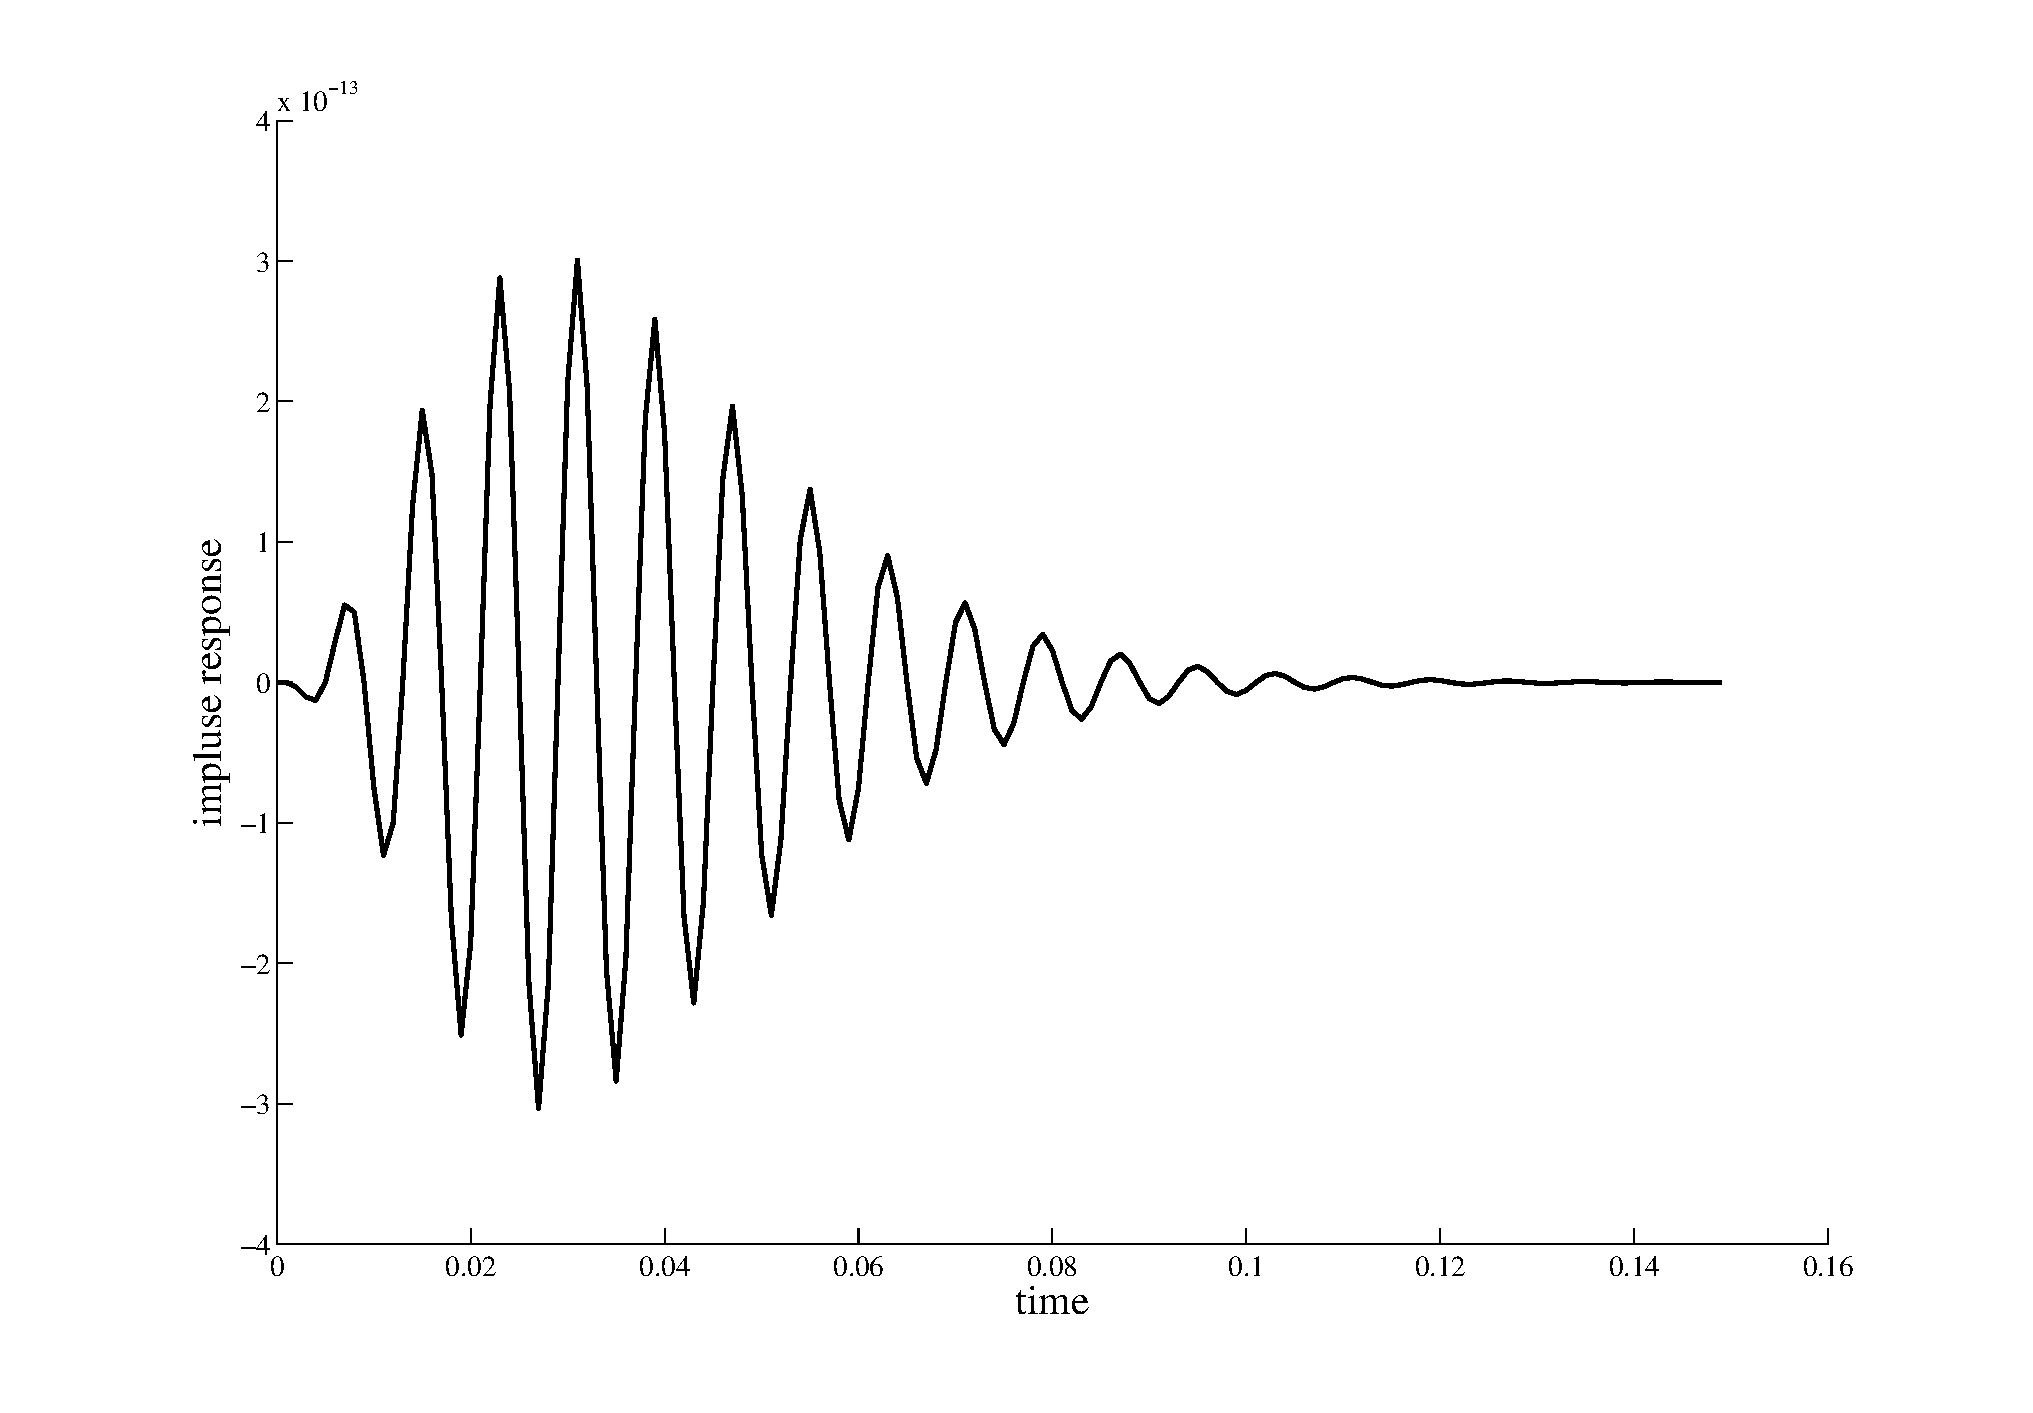
\includegraphics[width=0.8\textwidth]{figs/gtimr}
\caption{Gamma-tone~濾波器之脈衝響應(中心頻率為~$1000$~Hz)} 
\label{fig:gtimr}
\end{figure}

\begin{figure}[!htb]
\centering
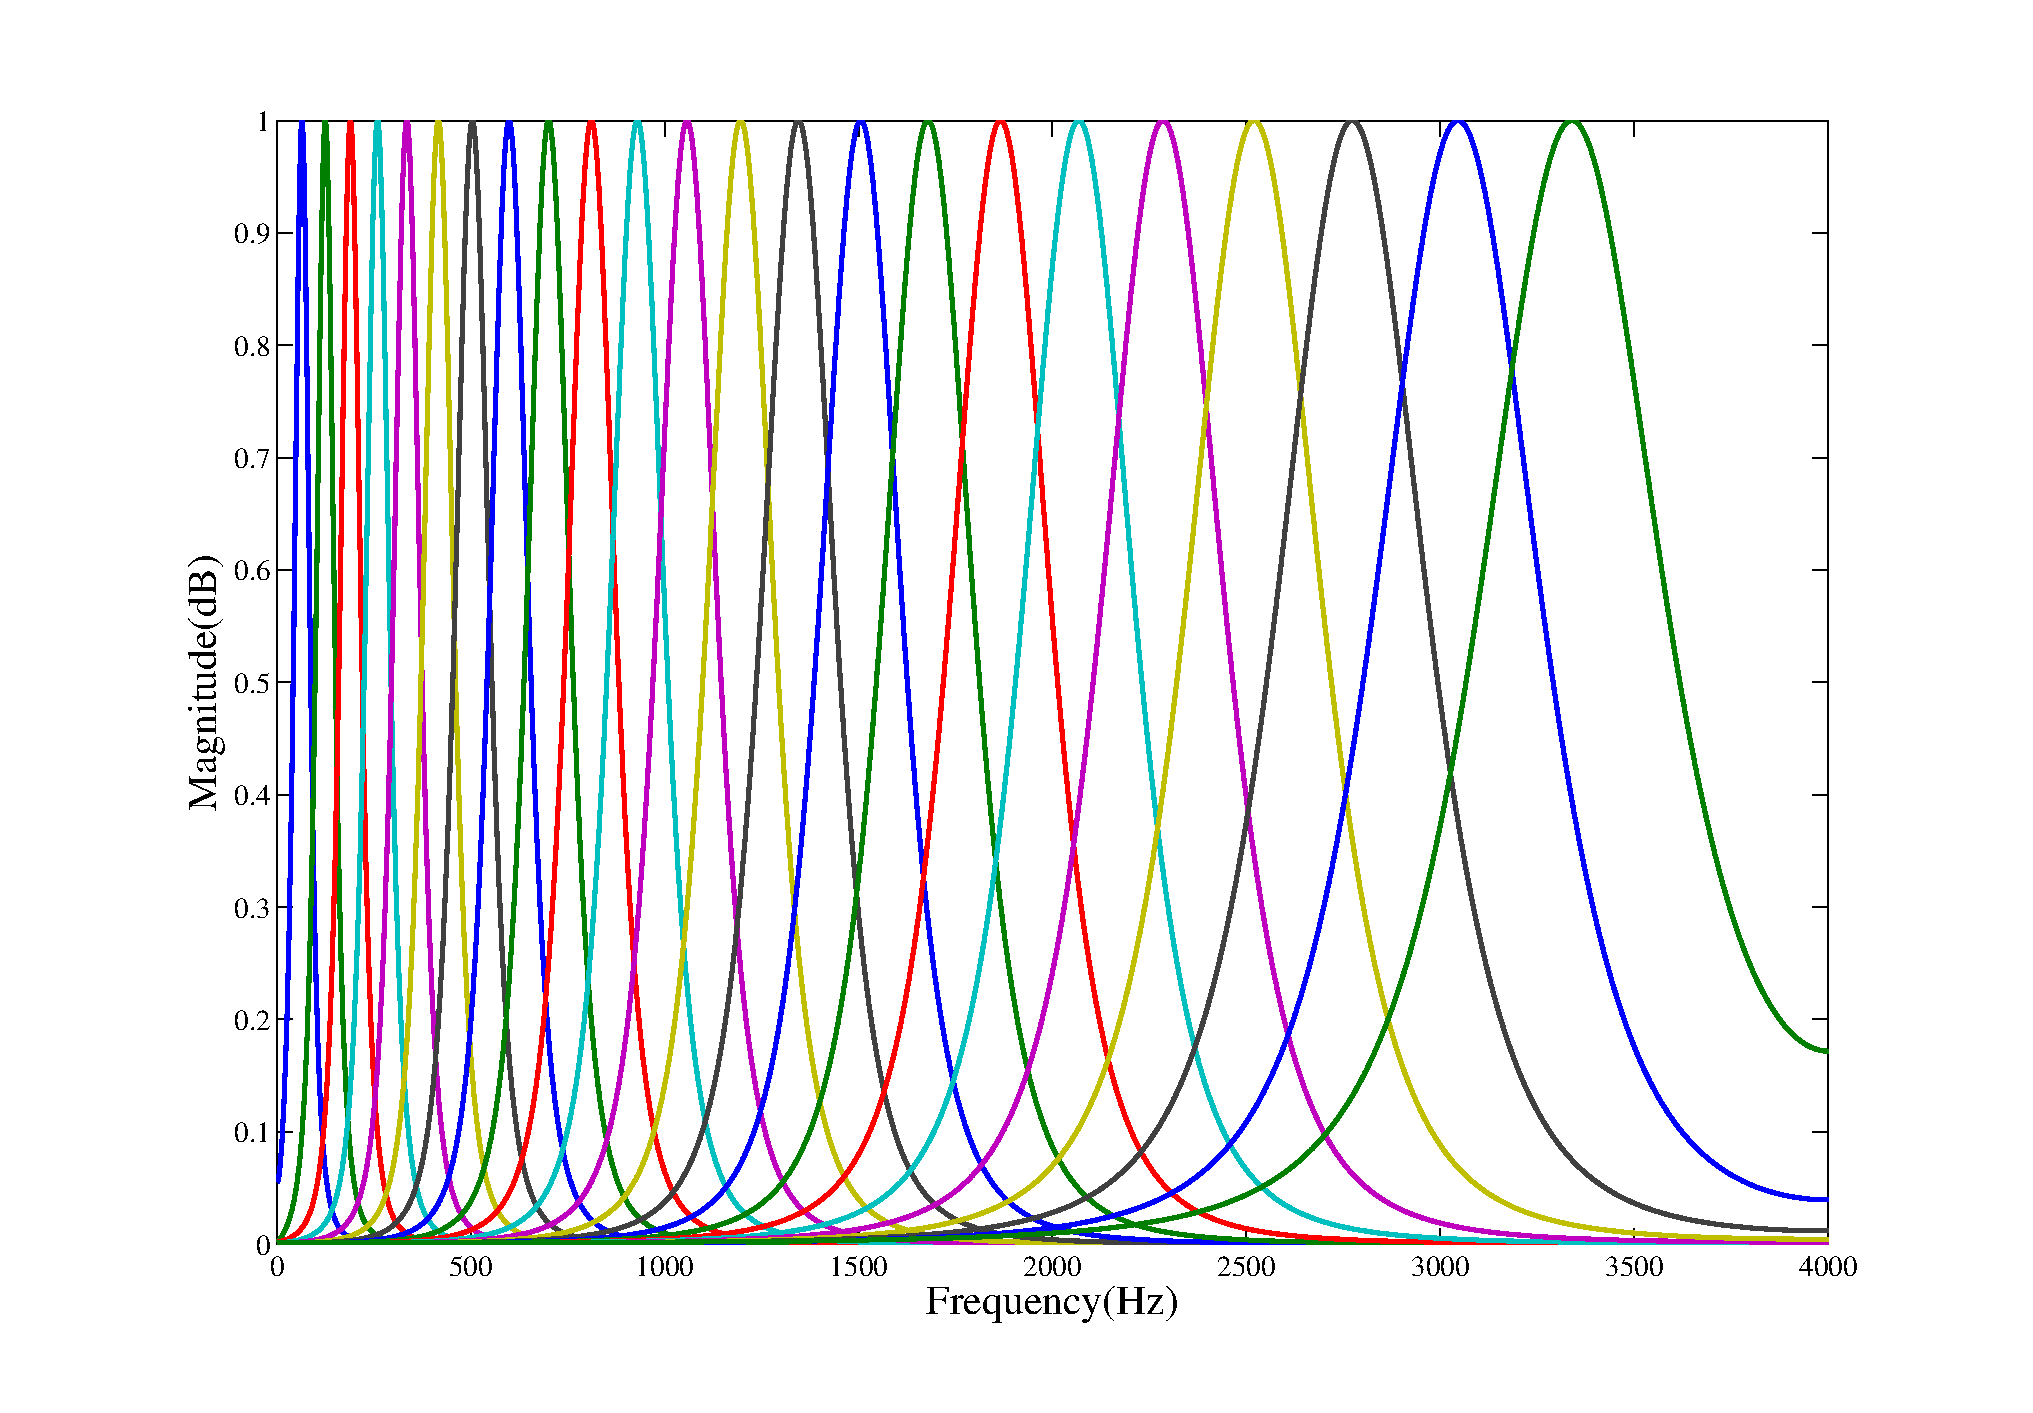
\includegraphics[width=0.8\textwidth]{figs/gafrqres}
\caption{Gamma-tone~濾波器之頻率響應} 
\label{fig:gafrqres}
\end{figure}

\subsection{Teager~能量評估法}
\label{sec:mte}
Teager~能量評估法是一種非線性能量計算的方法,
其主要目的在於增強語音訊號與噪音之間的能量差別。
將語音中穩定或半穩定~(語音部分)~予以強化,並且使不穩定的訊號~(雜訊部分)~的能量值衰減。
其連續時間的方程式表示為
\begin{equation}
\label{eq:teocont}
	\psi \left[ x(t) \right] = \left[  \frac{d}{dt} x(t) \right]^2 - x(t) \left[  \frac{d^2}{dt^2} x(t) \right].
\end{equation}
將方程式(\ref{eq:teocont})~轉換為離散型式,式子如下
\begin{equation}
\label{eq:teodis}
	\psi \left[ x(n)  \right] = \left[  x(n) \right]^2 - x(n+1)x(n-1).
\end{equation}
我們發現方程式(\ref{eq:teodis})~在處理一個音框前後兩端邊緣的取樣點會有超出邊界的問題,
因此將式子修改為
\begin{equation}
    \begin{aligned}
      & x[n] =  & \begin{cases} \left( x[n] \right)^2 - x[n] \cdot x[n+1], &\text{if $n=0$} \\  
					     \left( x[n] \right)^2 - x[n] \cdot x[n-1], &\text{if $n=N-1$} \\  
					     \left( x[n] \right)^2 -x[n+1] \cdot x[n-1],&\text{otherwise}.
	\end{cases} 
    \end{aligned}
 \end{equation}        

本論文中,我們將~GTF~各個頻帶的能量皆使用~Teager~能量評估法降低噪音的能量,使我們所擷取的特徵參數能夠更加具有噪音強健性。
